%\documentclass[12pt]{article}
%\usepackage[a4paper, margin=1in]{geometry} 
%\usepackage{graphicx} 
%\usepackage{hyperref}
%\usepackage{float}
%\usepackage{multicol}
%\usepackage{amsmath}
%\usepackage[ruled]{algorithm2e}
%\usepackage{amssymb}
%\usepackage[font=small, labelfont=bf]{caption}
%
%\begin{document}

%
% Needleman-Wunsch
%
\subsection{Needleman-Wunsch algorithm}
The method of using DP to solve global pairwise alignment is called the Needleman-Wunsch algorithm in the field of bioinformatics. 

%
% Complexity
%
\subsubsection*{Complexity}
\begin{itemize}
\item Time: O(nm)
\item Space: O(nm)
\end{itemize}

%
% Comparisons with other algorithms
%
\subsubsection*{Comparisons with other algorithms}
The Needleman-Wunsch algorithm is similar to several algorithms.
\\

\noindent
\textbf{Divide and conquer algorithms}

\noindent
Sub-solutions must be independent with divide and conquer.

\begin{figure}[H]
  \centering
      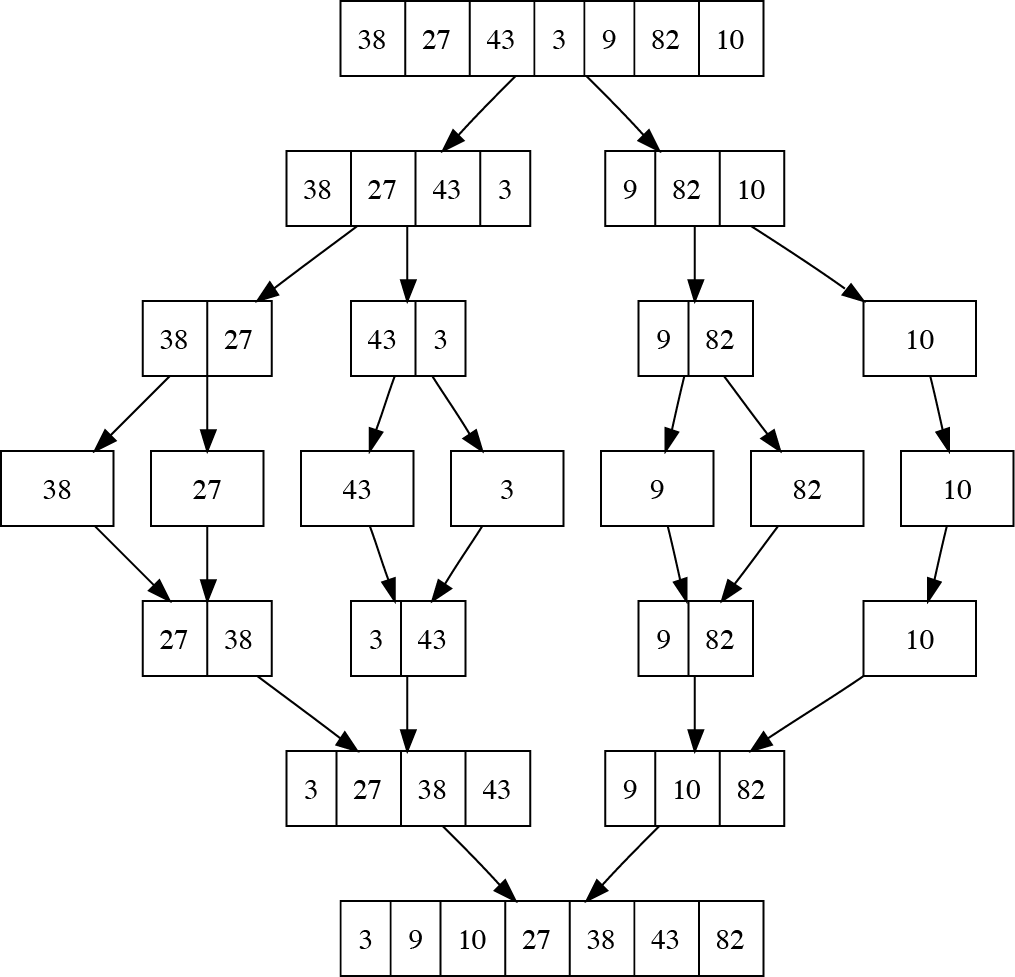
\includegraphics[width=0.25\textwidth]{fig02/Merge_sort_algorithm.png}
  \caption{Merge sort (source: \href{https://commons.wikimedia.org/w/index.php?curid=8004317}{VineetKumar, Wikimedia Commons})}
\end{figure}

\noindent
\textbf{Dijkstra's algorithm}

\noindent
Worst-case performance of Dijkstra: $O(|E|+|V|\log |V|)$

\begin{figure}[H]
  \centering
      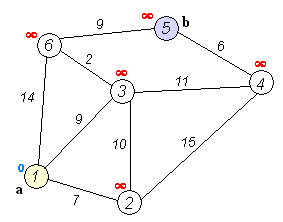
\includegraphics[width=0.25\textwidth]{fig02/Dijkstra.png}
  \caption{Dijkstra's algorithm (source: \href{https://commons.wikimedia.org/w/index.php?curid=6282617}{Ibmua, Wikimedia Commons})}
\end{figure}

%\end{document}
